% Options for packages loaded elsewhere
\PassOptionsToPackage{unicode}{hyperref}
\PassOptionsToPackage{hyphens}{url}
\PassOptionsToPackage{dvipsnames,svgnames,x11names}{xcolor}
\documentclass[
  11pt,
]{article}
\usepackage{xcolor}
\usepackage[margin=2.5cm]{geometry}
\usepackage{amsmath,amssymb}
\setcounter{secnumdepth}{-\maxdimen} % remove section numbering
\usepackage{iftex}
\ifPDFTeX
  \usepackage[T1]{fontenc}
  \usepackage[utf8]{inputenc}
  \usepackage{textcomp} % provide euro and other symbols
\else % if luatex or xetex
  \usepackage{unicode-math} % this also loads fontspec
  \defaultfontfeatures{Scale=MatchLowercase}
  \defaultfontfeatures[\rmfamily]{Ligatures=TeX,Scale=1}
\fi
\usepackage[]{charter}
\ifPDFTeX\else
  % xetex/luatex font selection
\fi
% Use upquote if available, for straight quotes in verbatim environments
\IfFileExists{upquote.sty}{\usepackage{upquote}}{}
\IfFileExists{microtype.sty}{% use microtype if available
  \usepackage[]{microtype}
  \UseMicrotypeSet[protrusion]{basicmath} % disable protrusion for tt fonts
}{}
\makeatletter
\@ifundefined{KOMAClassName}{% if non-KOMA class
  \IfFileExists{parskip.sty}{%
    \usepackage{parskip}
  }{% else
    \setlength{\parindent}{0pt}
    \setlength{\parskip}{6pt plus 2pt minus 1pt}}
}{% if KOMA class
  \KOMAoptions{parskip=half}}
\makeatother
\usepackage{graphicx}
\makeatletter
\newsavebox\pandoc@box
\newcommand*\pandocbounded[1]{% scales image to fit in text height/width
  \sbox\pandoc@box{#1}%
  \Gscale@div\@tempa{\textheight}{\dimexpr\ht\pandoc@box+\dp\pandoc@box\relax}%
  \Gscale@div\@tempb{\linewidth}{\wd\pandoc@box}%
  \ifdim\@tempb\p@<\@tempa\p@\let\@tempa\@tempb\fi% select the smaller of both
  \ifdim\@tempa\p@<\p@\scalebox{\@tempa}{\usebox\pandoc@box}%
  \else\usebox{\pandoc@box}%
  \fi%
}
% Set default figure placement to htbp
\def\fps@figure{htbp}
\makeatother
\setlength{\emergencystretch}{3em} % prevent overfull lines
\providecommand{\tightlist}{%
  \setlength{\itemsep}{0pt}\setlength{\parskip}{0pt}}
% ==========================================================================
%  IA na Sociedade — cabeçalho LaTeX (pdflatex)
%  Programa CiberExt 26-29 · FEELT38103
%  Adaptado de "AI in Society" (Universidade de Helsinque / Una Europa)
%  Licença: CC BY-NC-SA 4.0
% --------------------------------------------------------------------------
%  Espelha a identidade do ia-style.css: papel quente, tinta ardósia e a
%  faixa tricolor dos três eixos do curso (conceitos / aplicações / riscos).
% ==========================================================================

% ---------- Fontes ----------
% A serifada vem do build.sh, que passa  -V fontfamily=charter  ao pandoc.
% Aqui só acrescentamos a sem-serifa; ambas com fallback, porque nem toda
% instalação de LaTeX traz os mesmos pacotes.
\IfFileExists{helvet.sty}{\usepackage[scaled=0.90]{helvet}}{}
\usepackage{textcomp}
\IfFileExists{microtype.sty}{\usepackage{microtype}}{}

% ---------- Pacotes de layout ----------
\usepackage{xcolor}
\usepackage{tcolorbox}
\tcbuselibrary{skins,breakable}
\usepackage{titlesec}
\usepackage{fancyhdr}
\usepackage{enumitem}
\usepackage{amssymb}
\usepackage{booktabs}
\usepackage{array}
\usepackage{colortbl}
\usepackage{ragged2e}
\usepackage{fvextra}
\usepackage{newunicodechar}

% ---------- Caracteres Unicode que o pdflatex não conhece ----------
\newunicodechar{✓}{{\color{iaAplic}\checkmark}}
\newunicodechar{✅}{{\color{iaAplic}\checkmark}}
\newunicodechar{→}{\ensuremath{\rightarrow}}
\newunicodechar{←}{\ensuremath{\leftarrow}}
\newunicodechar{↔}{\ensuremath{\leftrightarrow}}
\newunicodechar{–}{--}
\newunicodechar{—}{---}
\newunicodechar{€}{\texteuro}
\newunicodechar{£}{\textsterling}
\newunicodechar{×}{\ensuremath{\times}}
\newunicodechar{≈}{\ensuremath{\approx}}
\newunicodechar{≥}{\ensuremath{\geq}}
\newunicodechar{≤}{\ensuremath{\leq}}
\newunicodechar{•}{\textbullet}
\newunicodechar{″}{''}
\newunicodechar{′}{'}

% ==========================================================================
%  PALETA — os mesmos valores do ia-style.css
% ==========================================================================
\definecolor{iaConceitos}{HTML}{24505C}   % petróleo — títulos, eixo 1
\definecolor{iaAplic}{HTML}{16746C}       % verdete  — subtítulos, eixo 2
\definecolor{iaRiscos}{HTML}{B45F14}      % açafrão  — destaques, eixo 3
\definecolor{iaAmeixa}{HTML}{77345F}      % links internos, termos técnicos
\definecolor{iaTinta}{HTML}{1F2933}       % corpo do texto
\definecolor{iaTintaFraca}{HTML}{5C6670}
\definecolor{iaRegra}{HTML}{E4DBCD}
\definecolor{iaBloco}{HTML}{F3EEE4}
\definecolor{iaNota}{HTML}{EAF1F0}
\definecolor{iaCaso}{HTML}{FCF3E6}
\definecolor{iaFilos}{HTML}{F7EFF4}

\color{iaTinta}

% ==========================================================================
%  ASSINATURA — faixa tricolor dos três eixos
% ==========================================================================
\newcommand{\faixaEixos}[1][\linewidth]{%
  \noindent
  \textcolor{iaConceitos}{\rule{0.3333#1}{4pt}}%
  \textcolor{iaAplic}{\rule{0.3333#1}{4pt}}%
  \textcolor{iaRiscos}{\rule{0.3333#1}{4pt}}%
  \par}

% ---------- Página de título ----------
\makeatletter
\newcommand{\subtitle}[1]{\gdef\@subtitle{#1}}
\providecommand{\@subtitle}{}
\def\@maketitle{%
  \newpage\null\vskip 1.5em%
  \faixaEixos
  \vskip 2.2em
  {\raggedright
    {\sffamily\bfseries\huge\color{iaConceitos}\@title\par}%
    \vskip 0.7em%
    {\sffamily\large\color{iaTintaFraca}\@subtitle\par}%
    \vskip 2em%
    {\color{iaRegra}\rule{\linewidth}{1pt}}%
    \vskip 1em%
    {\sffamily\small\color{iaTinta}\@author\par}%
    \vskip 0.5em%
    {\sffamily\footnotesize\color{iaTintaFraca}\@date\par}%
  }\par\vskip 2.5em}
\makeatother

% ==========================================================================
%  TÍTULOS DE SEÇÃO
% ==========================================================================
\titleformat{\section}[block]
  {\sffamily\Large\bfseries\color{iaConceitos}}
  {\thesection}{0.7em}{}
  [{\vspace{2pt}\color{iaRegra}\titlerule[1.2pt]}]
\titleformat{\subsection}
  {\sffamily\large\bfseries\color{iaAplic}}
  {\thesubsection}{0.6em}{}
\titleformat{\subsubsection}
  {\sffamily\normalsize\bfseries\color{iaRiscos}}
  {\thesubsubsection}{0.5em}{}
\titleformat{\paragraph}[runin]
  {\sffamily\small\bfseries\color{iaRiscos}}
  {}{0em}{}

\titlespacing*{\section}{0pt}{2.6ex plus 1ex minus .2ex}{1.3ex plus .2ex}
\titlespacing*{\subsection}{0pt}{2.2ex plus 1ex minus .2ex}{1ex plus .2ex}

% ==========================================================================
%  CABEÇALHO E RODAPÉ
% ==========================================================================
\setlength{\headheight}{24pt}
\renewcommand{\sectionmark}[1]{\markboth{#1}{}}
\pagestyle{fancy}
\fancyhf{}
\renewcommand{\headrulewidth}{0.6pt}
\renewcommand{\footrulewidth}{0pt}
\fancyhead[L]{\sffamily\footnotesize\color{iaAplic}Ética da IA}
\fancyhead[R]{\sffamily\footnotesize\color{iaAplic}\nouppercase{\leftmark}}
\fancyfoot[C]{\sffamily\footnotesize\color{iaConceitos}\thepage}
\renewcommand{\headrule}{%
  \hbox to\headwidth{\color{iaRegra}\leaders\hrule height \headrulewidth\hfill}}

% ==========================================================================
%  TEXTO CORRIDO
% ==========================================================================
\linespread{1.08}
\setlength{\parskip}{0.55em}
\setlength{\parindent}{0pt}
\emergencystretch=3em
\hbadness=10000

% ---------- Termos técnicos / código inline ----------
\let\oldtexttt\texttt
\renewcommand{\texttt}[1]{{\color{iaAmeixa}\small\ttfamily #1}}

% ---------- Blocos verbatim ----------
\fvset{breaklines=true,breakanywhere=true,fontsize=\small}

% ---------- Blocos de código (ambiente Shaded do pandoc) ----------
% O pandoc só pré-define o ambiente Shaded quando o markdown tem bloco de
% código; nos capítulos sem código ele não existe, e \renewenvironment
% incondicional falharia com "Environment Shaded undefined". \@ifundefined
% escolhe \newenvironment ou \renewenvironment conforme o caso.
\makeatletter
\@ifundefined{Shaded}{\newenvironment{Shaded}}{\renewenvironment{Shaded}}
  {\begin{tcolorbox}[
      breakable, enhanced jigsaw, rounded corners,
      arc=3pt, boxrule=0pt, frame hidden,
      colback=iaBloco,
      borderline west={3pt}{0pt}{iaAmeixa},
      left=10pt, right=8pt, top=6pt, bottom=6pt,
      before skip=9pt, after skip=9pt]}
  {\end{tcolorbox}}
\makeatother

% ---------- Citações: caixa de caso ----------
\renewenvironment{quote}
  {\begin{tcolorbox}[
      breakable, enhanced jigsaw, rounded corners,
      arc=3pt, boxrule=0pt, frame hidden,
      colback=iaCaso,
      borderline west={3pt}{0pt}{iaRiscos},
      left=12pt, right=10pt, top=9pt, bottom=9pt,
      before skip=9pt, after skip=9pt]}
  {\end{tcolorbox}}

% ==========================================================================
%  BLOCOS DE APOIO
%  No markdown, escreva:   ::: nota   ...texto...   :::
%  O pandoc converte fenced_divs para os ambientes abaixo.
% ==========================================================================
\newtcolorbox{iabox}[3]{
  breakable, enhanced jigsaw, rounded corners,
  arc=3pt, boxrule=0pt, frame hidden,
  colback=#2,
  borderline west={3pt}{0pt}{#1},
  left=12pt, right=10pt, top=9pt, bottom=9pt,
  before skip=11pt, after skip=11pt,
  before upper={\setlength{\parskip}{0.5em}\setlength{\parindent}{0pt}},
  title={\sffamily\bfseries\footnotesize\textcolor{#1}{\MakeUppercase{#3}}},
  attach title to upper={\par\vspace{5pt}},
  fonttitle=\normalfont}

% Cada ambiente aceita um titulo opcional entre colchetes, vindo do
% atributo data-titulo do markdown:   \begin{filosofia}[Titulo] ... \end{filosofia}
% Os quatro primeiros espelham os icones do material original.
\newenvironment{filosofia}[1][Conceito filosofico]{\begin{iabox}{iaAmeixa}{iaFilos}{#1}}{\end{iabox}}
\newenvironment{tecnica}[1][Nota tecnica]{\begin{iabox}{iaConceitos}{iaNota}{#1}}{\end{iabox}}
\newenvironment{contexto}[1][Contexto]{\begin{iabox}{iaAplic}{iaBloco}{#1}}{\end{iabox}}
\newenvironment{definicao}[1][Definicao]{\begin{iabox}{iaRiscos}{iaCaso}{#1}}{\end{iabox}}

\newenvironment{nota}[1][Nota]{\begin{iabox}{iaConceitos}{iaNota}{#1}}{\end{iabox}}
\newenvironment{caso}[1][Caso]{\begin{iabox}{iaRiscos}{iaCaso}{#1}}{\end{iabox}}
\newenvironment{reflexao}[1][Para pensar]{\begin{iabox}{iaAplic}{iaBloco}{#1}}{\end{iabox}}
\newenvironment{licenca}
  {\par\vspace{2em}\faixaEixos\par\vspace{0.8em}
   \begingroup\sffamily\scriptsize\color{iaTintaFraca}}
  {\endgroup\par}

% ==========================================================================
%  LISTAS
% ==========================================================================
\setlist[itemize]{leftmargin=1.4em, itemsep=2pt, topsep=4pt, parsep=0pt}
\setlist[enumerate]{leftmargin=1.7em, itemsep=2pt, topsep=4pt, parsep=0pt}
\renewcommand{\labelitemi}{\textcolor{iaRiscos}{\textbullet}}
\renewcommand{\labelitemii}{\textcolor{iaAplic}{--}}

% ==========================================================================
%  TABELAS
% ==========================================================================
\renewcommand{\arraystretch}{1.3}
\arrayrulecolor{iaRegra}

% ==========================================================================
%  RÓTULOS EM PORTUGUÊS
%  Definidos aqui (e não via -V na linha de comando) porque acentos passados
%  como argumento dependem do locale do terminal e podem se corromper.
% ==========================================================================
\renewcommand{\contentsname}{Sumário}
\renewcommand{\refname}{Referências}
\renewcommand{\figurename}{Figura}
\renewcommand{\tablename}{Tabela}
\usepackage{bookmark}
\IfFileExists{xurl.sty}{\usepackage{xurl}}{} % add URL line breaks if available
\urlstyle{same}
% fallback for those not using the hyperref driver hyperxmp:
\makeatletter
\@ifundefined{xmpquote}{\newcommand{\xmpquote}[1]{#1}}{}
\makeatother
\hypersetup{
  pdftitle={Ética da Inteligência Artificial},
  colorlinks=true,
  linkcolor={iaAmeixa},
  filecolor={Maroon},
  citecolor={Blue},
  urlcolor={iaRiscos},
  pdfcreator={LaTeX via pandoc}}

\title{Ética da Inteligência Artificial}
\usepackage{etoolbox}
\makeatletter
\providecommand{\subtitle}[1]{% add subtitle to \maketitle
  \apptocmd{\@title}{\par {\large #1 \par}}{}{}
}
\makeatother
\subtitle{Capítulo 5: Direitos humanos --- a IA deve respeitá-los e
promovê-los?}
\author{Tradução e adaptação para o português: José Lucas Lira Bizil,
Fernando Mazzeto Lisboa Lima e Matheus da Silva Fernandes\\
Programa CiberExt 26-29 · FEELT38103 · Universidade Federal de
Uberlândia\\
Original: \emph{Ethics of AI}, Universidade de Helsinque}
\date{2026}

\begin{document}
\maketitle

{
\hypersetup{linkcolor=iaConceitos}
\setcounter{tocdepth}{3}
\tableofcontents
}
\section{Capítulo 5: Direitos humanos --- a IA deve respeitá-los e
promovê-los?}\label{capuxedtulo-5-direitos-humanos-a-ia-deve-respeituxe1-los-e-promovuxea-los}

\begin{nota}[Sobre este capítulo]

\textbf{Eixo:} Conceitos, Aplicações e Riscos

Os direitos humanos são o alicerce das diretrizes éticas de IA. Este
capítulo examina privacidade, segurança e inclusão, o RGPD e as técnicas
de anonimização, a divisão de gênero na tecnologia e os direitos
específicos das crianças.

\end{nota}

\subsection{I. Introdução}\label{i.-introduuxe7uxe3o}

Durante a pandemia de covid-19, governos tiveram dificuldade para
encontrar estratégias eficazes de saída do confinamento de forma segura.
Segundo epidemiologistas, reabrir a sociedade exige rastreamento,
monitoramento e acompanhamento eficientes. Em muitos casos, isso levou
ao uso de diversos aplicativos de rastreamento. Esses aplicativos
levantaram várias preocupações com privacidade e segurança. Críticos os
viram como os primeiros passos rumo à vigilância algorítmica dos
cidadãos.

Em Londres, as autoridades decidiram tentar algo novo. Junto com
cientistas, desenvolveram métodos para ``capturar a atividade em
Londres'' e assim compreender melhor o nível de atividade da cidade. Num
projeto chamado
\href{https://www.turing.ac.uk/research/research-projects/project-odysseus-understanding-london-busyness-and-exiting-lockdown}{Odysseus},
as autoridades obtêm informações sobre a distribuição de atividades em
Londres combinando algoritmos de aprendizado de máquina (\emph{machine
learning}), análise estatística de séries temporais e processamento de
imagens. Essa informação sobre a atividade nas ruas de Londres pode ser
usada para a reabertura segura das vias e para o planejamento de saúde
pública.

\begin{figure}
\centering
\pandocbounded{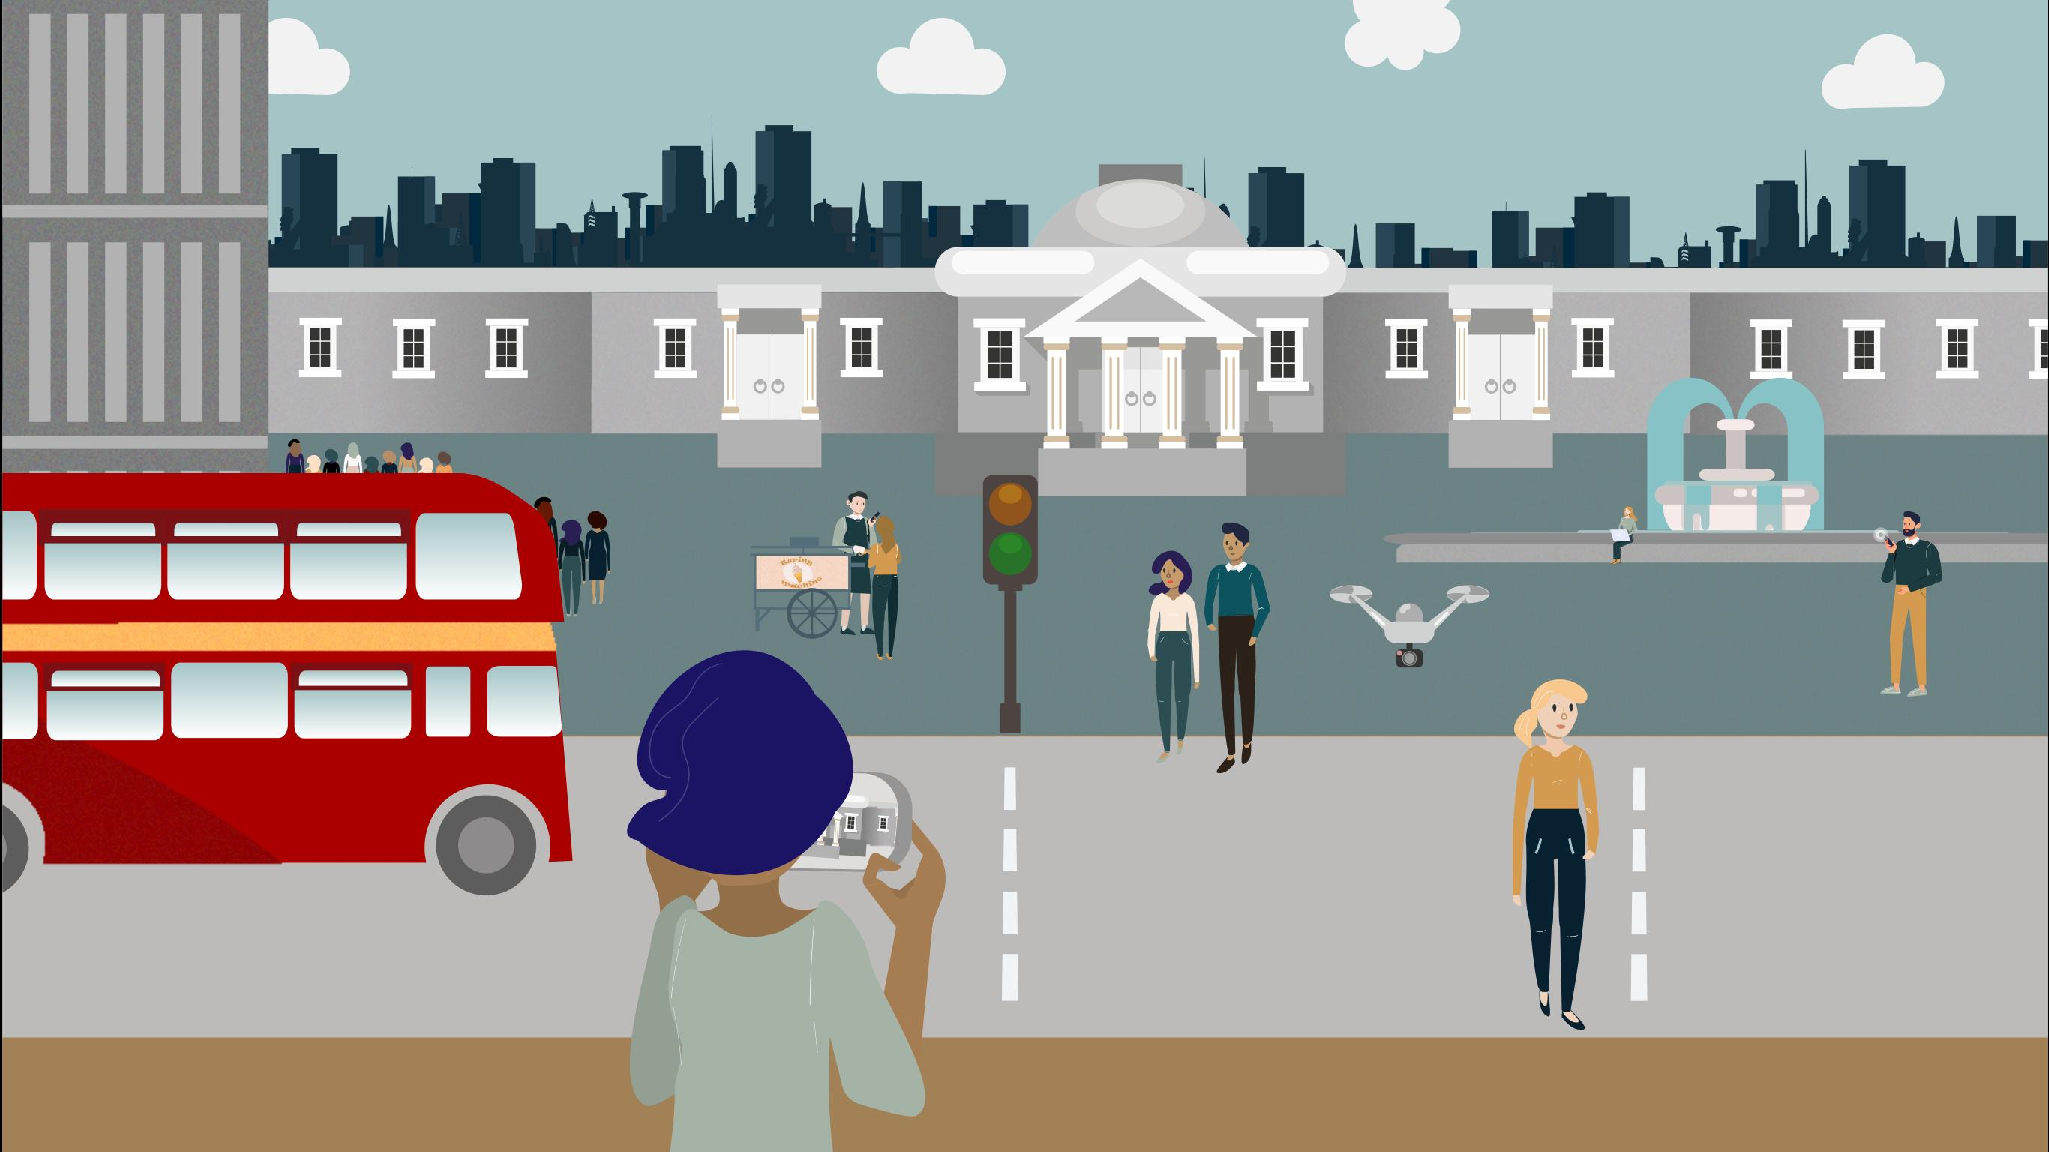
\includegraphics[keepaspectratio,alt={Atividade em Londres}]{img/london-01.pdf}}
\caption{Atividade em Londres}
\end{figure}

No Odysseus, os dados vêm de uma ampla gama de fontes. O projeto combina
dados agregados e anonimizados de telefonia móvel, transações
anonimizadas de cartão de crédito, dados de navegação por satélite e
dados de sensores e câmeras de trânsito nas ruas. Esses dados são usados
para criar contagens de veículos, ciclistas e pedestres, e para indicar
a densidade e os efeitos do distanciamento social. Atenção especial é
dada à anonimização, de modo que indivíduos não possam ser
identificados.

Neste capítulo, vamos olhar para os direitos humanos. O direito a um
ambiente seguro é um deles. O Odysseus é um exemplo de como a IA pode
ser usada de maneira que respeite e promova o direito à segurança ou a
um ambiente saudável. Ao mesmo tempo, o projeto precisa levar em conta
outros direitos --- como o direito à privacidade. Em Londres, essas
preocupações foram levadas a sério. Para garantir a privacidade, o
Odysseus é projetado de modo que todos os dados sejam anonimizados e que
indivíduos não possam ser identificados nas imagens captadas pelas
câmeras de trânsito.

Privacidade e segurança atraíram muita atenção da mídia. São
importantes, mas é necessário considerar também o impacto da IA sobre
todo o espectro de direitos e liberdades fundamentais. Como a IA
impactará o direito à educação e ao trabalho, ou a um julgamento justo,
a eleições justas e abertas, à liberdade de expressão, à reunião e à
manifestação? E quanto a grupos específicos, como as crianças? Mas,
primeiro, discutamos o que são direitos humanos.

\subsection{II. O que são direitos
humanos?}\label{ii.-o-que-suxe3o-direitos-humanos}

Os direitos humanos formam a base das atuais diretrizes e princípios
éticos de IA. Isso os torna um componente fundamental da ética
contemporânea da IA. Como direitos, os direitos humanos são
\textbf{universais}: todos os seres humanos têm direito a eles. Não é
preciso ser um tipo específico de pessoa ou membro de alguma comunidade
específica para tê-los.

Os direitos humanos são \textbf{normas} que protegem todas as pessoas,
em qualquer lugar, contra abusos políticos, jurídicos e sociais.
Incluem:

\begin{itemize}
\tightlist
\item
  \textbf{Direitos civis e políticos}, como o direito à vida, à
  liberdade e à propriedade, a liberdade de expressão, a busca da
  felicidade e a igualdade perante a lei;
\item
  \textbf{Direitos sociais, culturais e econômicos}, incluindo o direito
  de participar da ciência e da cultura, o direito ao trabalho e o
  direito à educação.
\end{itemize}

O papel dos direitos humanos é proteger a capacidade das pessoas de
formar, interpretar e perseguir suas próprias concepções de uma vida que
valha a pena --- não se trata apenas da capacidade de viver ``em
liberdade, felicidade e bem-estar''.

\begin{nota}[O que é um direito humano?]

Um direito humano é uma norma que pode existir em diferentes níveis:

\begin{itemize}
\tightlist
\item
  uma norma compartilhada das moralidades humanas efetivas;
\item
  uma norma moral justificada, apoiada por razões fortes;
\item
  um direito legal em nível nacional (onde pode ser chamado de direito
  ``civil'' ou ``constitucional'');
\item
  um direito legal no âmbito do direito internacional.
\end{itemize}

\textbf{O que é a Declaração Universal dos Direitos Humanos?}

A
\href{https://www.un.org/en/about-us/universal-declaration-of-human-rights}{Declaração
Universal dos Direitos Humanos} (DUDH) é um documento redigido por
representantes com diferentes formações jurídicas e culturais, de todas
as regiões do mundo. A declaração foi proclamada pela Assembleia Geral
das Nações Unidas em Paris, em 10 de dezembro de 1948 (resolução 217 A
da Assembleia Geral), como padrão comum de realizações para todos os
povos e todas as nações.

\end{nota}

Conceitualmente, os direitos humanos fundam-se na agência e na autonomia
(Gewirth, 1982). Têm prioridade ética: se entram em concorrência com
outras considerações, como riqueza econômica, estabilidade nacional ou
algum outro fator, os direitos humanos devem ser priorizados. No
contexto da IA, essa priorização implica os seguintes requisitos:

\begin{itemize}
\tightlist
\item
  aplicações de IA que possam claramente violar direitos humanos não
  devem ser usadas;
\item
  aplicações de IA que impeçam as pessoas de gozar de seus direitos
  humanos, ou que ativamente as coloquem em risco de violação, não devem
  ser usadas.
\end{itemize}

Contudo, os direitos humanos têm certas propriedades sensíveis ao
contexto, que permitem priorizar um direito humano específico quando
necessário. Alguns direitos são mais fundamentais do que outros. Por
exemplo, quando o direito à vida conflita com o direito à privacidade, o
direito à privacidade geralmente será superado.

Nos últimos anos, preocupações com privacidade e segurança dominaram a
discussão sobre IA e direitos humanos. Combinações emergentes de análise
de \emph{big data}, tecnologias de vigilância e métodos de
reconhecimento biométrico em desenvolvimento receberam atenção
significativa da mídia e das políticas públicas. Também o direito à
igualdade e à inclusão suscitou bastante discussão pública. Na próxima
seção, examinaremos brevemente esses debates.

\subsection{III. Exemplos de direitos humanos: privacidade, segurança e
inclusão}\label{iii.-exemplos-de-direitos-humanos-privacidade-seguranuxe7a-e-inclusuxe3o}

\subsubsection{Privacidade}\label{privacidade}

Preocupações com privacidade são levantadas, por exemplo, por registros
digitais que contêm informações capazes de permitir a inferência de
atributos sensíveis (idade, gênero ou orientação sexual), preferências
ou posições religiosas e políticas. Dados biométricos também levantam
preocupações, pois podem revelar detalhes de saúde física e mental.
Muitas vezes, a preocupação real não é o dado em si, mas o modo como ele
pode ser usado para manipular, afetar ou prejudicar uma pessoa.

Eticamente, a privacidade relaciona-se à autonomia e à integridade
pessoais. Seguindo os princípios estabelecidos por John Locke, o direito
de controlar nossa própria vida pessoal tem sido visto como central para
nossa autonomia. Se esse direito é retirado, viola-se algo fundamental
de nossa integridade psicológica e moral.

\begin{filosofia}[O que são os "seus" dados?]

Muitos propuseram o princípio de que as pessoas devem ter controle sobre
os próprios dados --- e de que os dados a seu respeito não devem poder
ser usados para prejudicá-las ou discriminá-las. Segundo alguns, esse
direito ao ``controle pleno sobre os próprios dados'' deveria ser um
direito humano.

Mas o que exatamente são os ``seus dados''? São os dados brutos, ou os
dados coletados e analisados? Se os dados são usados para finalidades
secundárias, ainda são seus? Ou, como observam Wachter e Mittelstadt
(\href{https://osf.io/preprints/lawarxiv/mu2kf/}{2019}), o conteúdo das
inferências que podem ser extraídas de seus dados pertence aos ``seus
dados''?

Wachter e Mittelstadt (2019) propõem que o direito ao controle dos
próprios dados seja reformulado como um direito a ``inferências
razoáveis''. Segundo eles, é crucial que possamos controlar também as
``inferências de alto risco'' que podem ser feitas sobre nós por meio de
análise de \emph{big data}. Essas inferências invadem a privacidade ou
danificam a reputação, ou têm baixa verificabilidade (no sentido de
serem preditivas ou baseadas em opinião), sendo ao mesmo tempo usadas
para decisões importantes.

\end{filosofia}

\begin{figure}
\centering
\pandocbounded{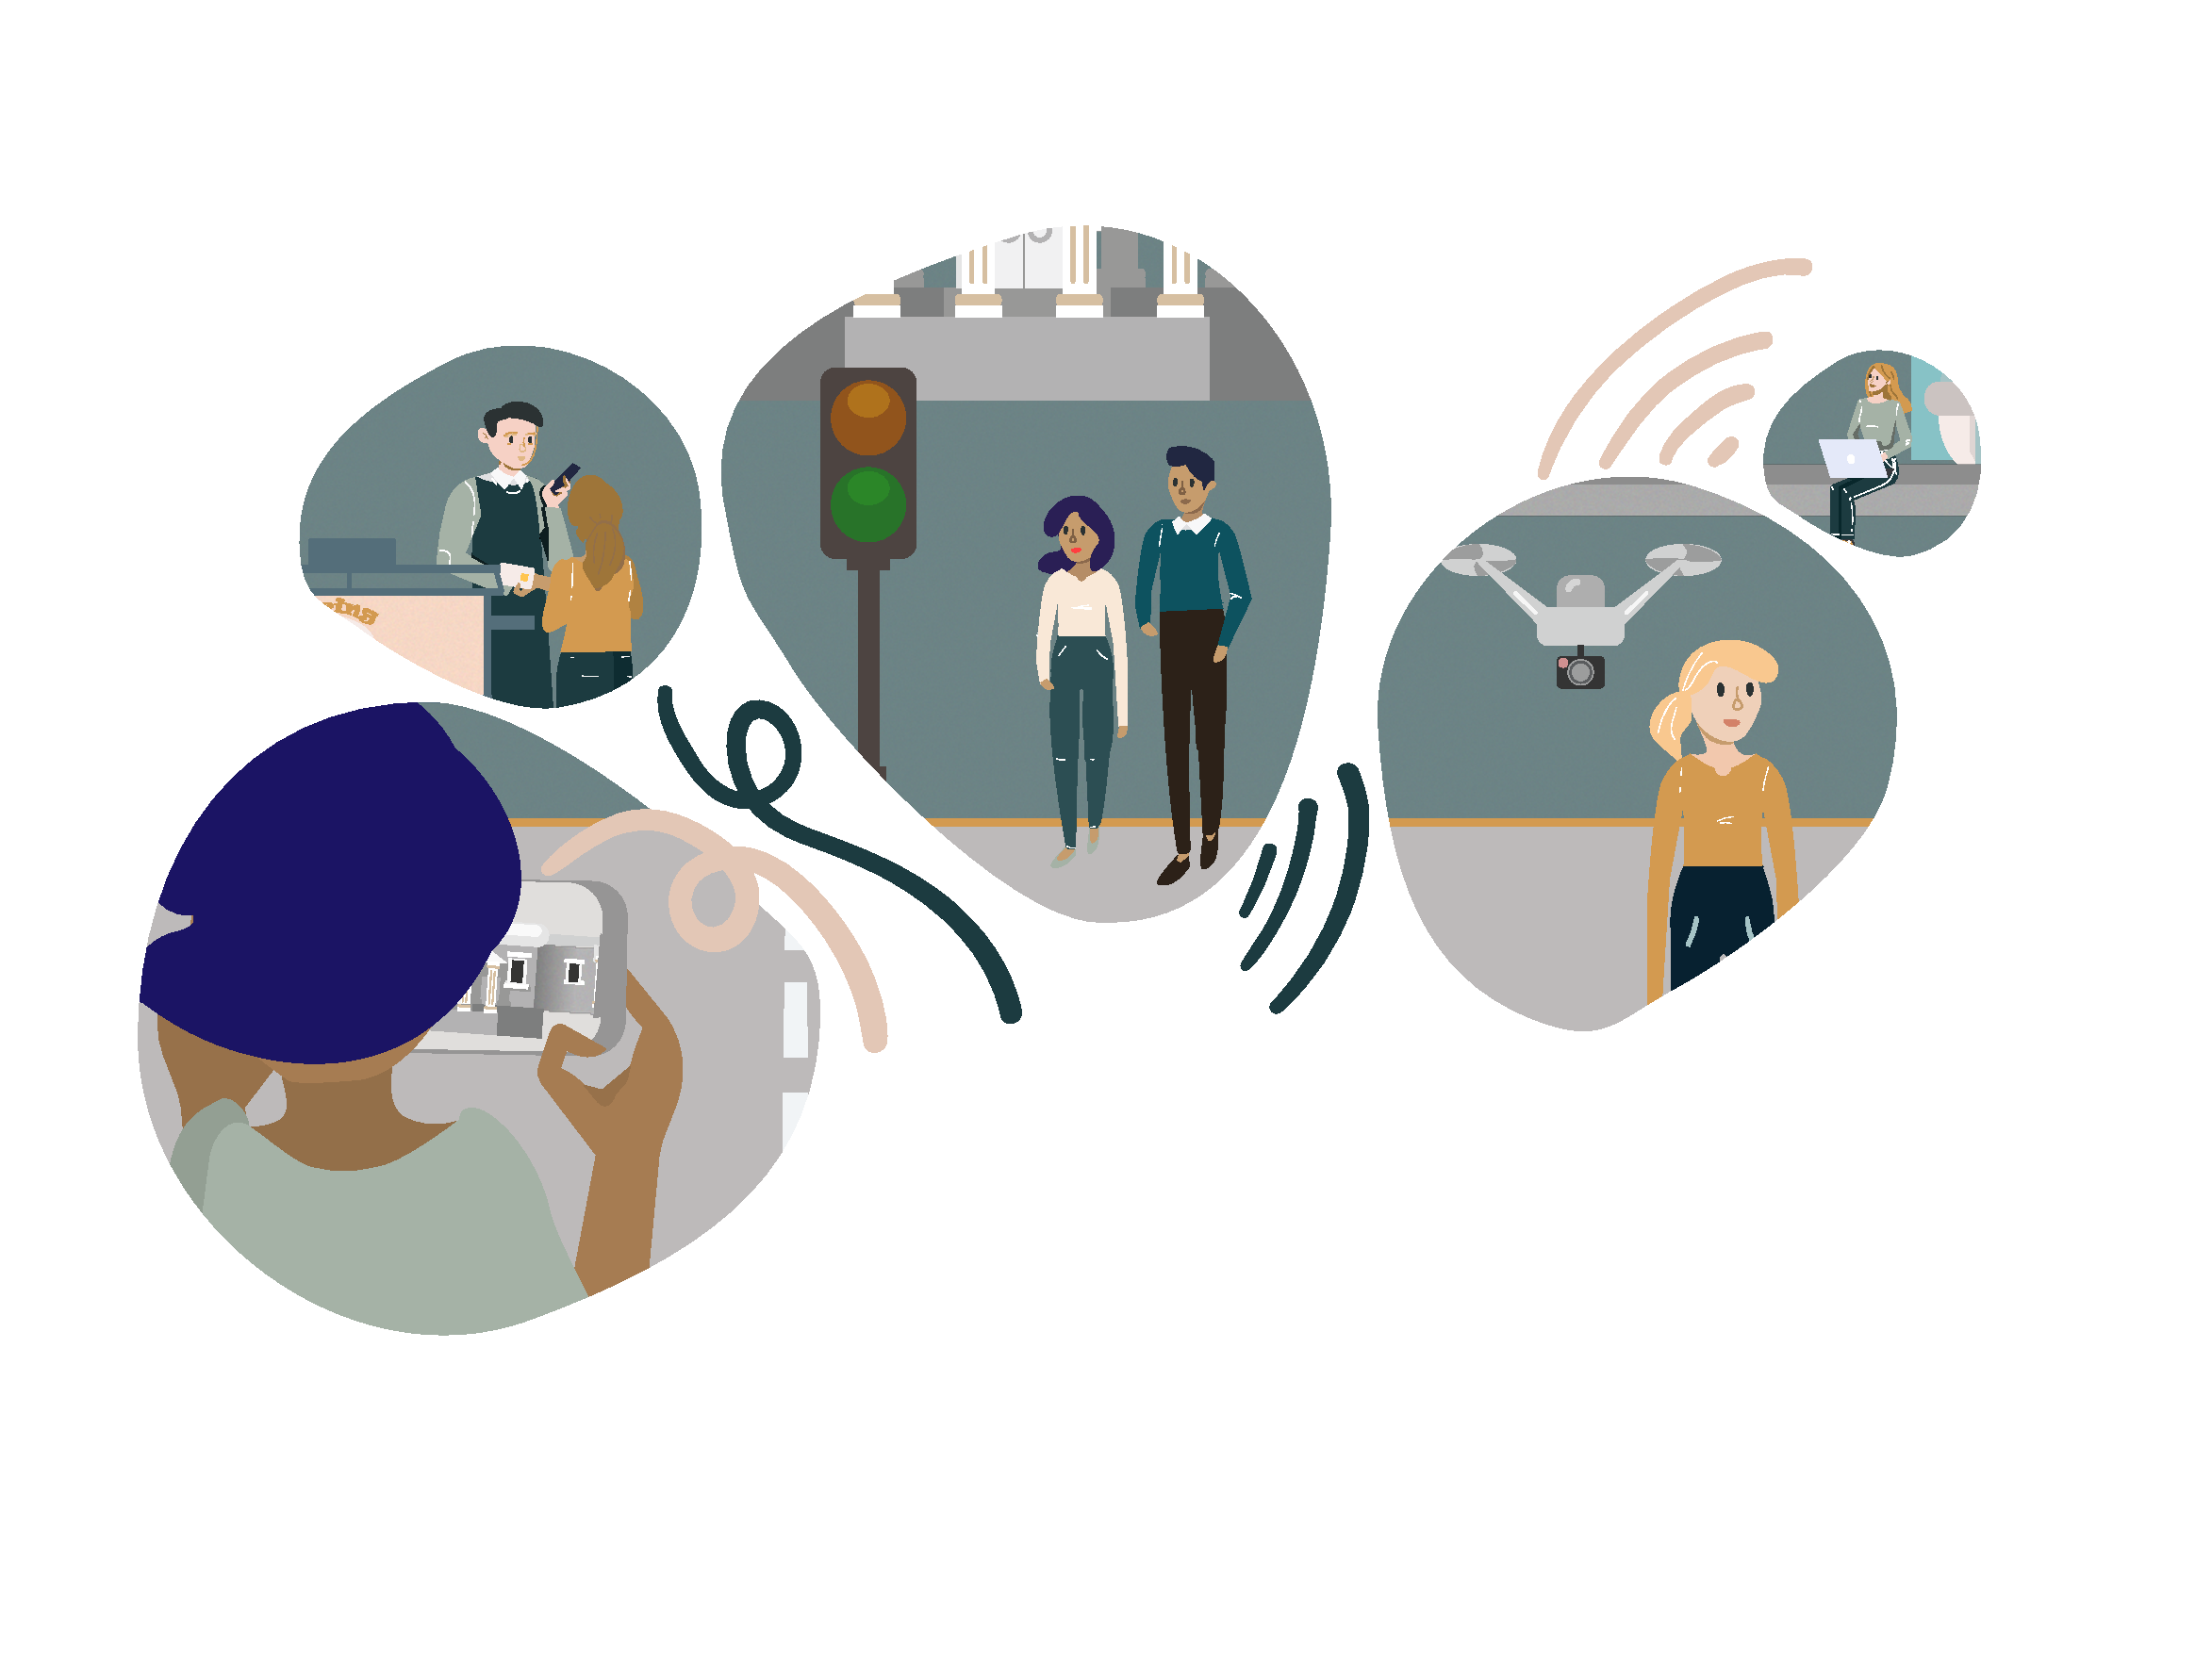
\includegraphics[keepaspectratio,alt={Detalhe do mapa de atividade}]{img/london-zoom.pdf}}
\caption{Detalhe do mapa de atividade}
\end{figure}

\paragraph{O RGPD}\label{o-rgpd}

O Regulamento Geral sobre a Proteção de Dados
(\href{https://gdpr.eu/what-is-gdpr/}{RGPD}, ou GDPR em inglês) é um
marco jurídico. Estabelece diretrizes para a coleta e o processamento de
dados pessoais de indivíduos que vivem na União Europeia.

O objetivo do RGPD é dar aos indivíduos controle sobre seus dados
pessoais. Qualquer informação relativa a um indivíduo que possa ser
direta ou indiretamente identificado é ``dado pessoal''. Isso inclui
nomes, números de identificação social e endereços de e-mail.
Informações de localização, dados biométricos, etnia, gênero,
\emph{cookies} de navegação e crenças políticas ou religiosas também
podem ser dados pessoais. Dados pseudonimizados (que não identificam
diretamente um indivíduo, mas podem ser a ele conectados) também podem
se enquadrar na definição, se for fácil individualizar alguém a partir
deles.

O titular dos dados deve dar consentimento específico e inequívoco para
o processamento. Os consentimentos devem ser ``livres, específicos,
informados e inequívocos''. Titulares podem retirar a qualquer momento
um consentimento previamente dado. Crianças menores de 13 anos só podem
consentir com autorização dos pais.

O RGPD reconhece diversos direitos de privacidade para os titulares, com
o objetivo de lhes dar mais controle sobre os dados. Alguns deles:

\begin{itemize}
\tightlist
\item
  o direito de ser informado (a pessoa deve ser avisada sobre o uso de
  seus dados pessoais);
\item
  o direito de acesso (deve ser explicado como os dados pessoais de
  alguém são usados);
\item
  o direito de retificação (a pessoa tem direito ao esquecimento e à
  exclusão dos dados);
\item
  o direito de restringir o processamento (a pessoa pode negar o uso de
  seus dados pessoais).
\end{itemize}

Se você processa dados, o RGPD exige que o faça segundo princípios de
proteção e responsabilização (\emph{accountability}). Esses princípios
devem ser considerados no projeto de qualquer novo produto ou atividade.
São eles:

\begin{itemize}
\tightlist
\item
  \textbf{Licitude, lealdade e transparência:} o processamento deve ser
  lícito, leal e transparente para o titular.
\item
  \textbf{Limitação da finalidade:} os dados devem ser processados para
  as finalidades legítimas especificadas explicitamente ao titular no
  momento da coleta.
\item
  \textbf{Minimização dos dados:} deve-se coletar e processar apenas a
  quantidade de dados absolutamente necessária para as finalidades
  especificadas.
\item
  \textbf{Exatidão:} os dados pessoais devem ser mantidos exatos e
  atualizados.
\item
  \textbf{Limitação da conservação:} dados de identificação pessoal só
  podem ser armazenados pelo tempo necessário à finalidade especificada.
\item
  \textbf{Integridade e confidencialidade:} o processamento deve ser
  feito de modo a assegurar segurança, integridade e confidencialidade
  adequadas (por exemplo, com criptografia).
\item
  \textbf{Responsabilização:} o controlador dos dados é responsável por
  poder demonstrar conformidade com todos esses princípios.
\end{itemize}

Segundo o RGPD, quem processa dados também é obrigado a tratá-los com
segurança por meio de ``medidas técnicas e organizacionais
apropriadas''.

\paragraph{Como proteger a privacidade --- métodos de
anonimização}\label{como-proteger-a-privacidade-muxe9todos-de-anonimizauxe7uxe3o}

O RGPD permite que organizações coletem dados anonimizados sem
consentimento, os usem para qualquer finalidade e os armazenem por tempo
indefinido --- desde que removam todos os identificadores. Há várias
técnicas de anonimização, entre elas:

\begin{itemize}
\item
  \textbf{Generalização} é um método que remove deliberadamente parte
  dos dados para torná-los menos identificáveis. Os dados podem ser
  transformados num conjunto de faixas ou numa área ampla com limites
  apropriados. É possível remover, por exemplo, o endereço da rua
  mantendo a informação do nome da cidade. Assim, eliminam-se alguns
  identificadores preservando certo grau de exatidão.
\item
  \textbf{Pseudonimização} é um método de gestão de dados e de
  desidentificação que substitui identificadores privados --- nomes,
  códigos de identificação --- por identificadores falsos ou
  pseudônimos, por exemplo trocando o identificador ``Santeri'' por
  ``Saara''. A pseudonimização preserva a exatidão estatística e a
  integridade dos dados. Os dados modificados podem ser usados
  protegendo ao mesmo tempo a privacidade.
\item
  \textbf{Dados sintéticos} é um método que usa conjuntos de dados
  artificiais criados, em vez de alterar o conjunto original. O processo
  envolve criar modelos estatísticos com base nos padrões encontrados no
  conjunto original. Podem-se usar desvios-padrão, medianas, regressão
  linear ou outras técnicas estatísticas para gerar os dados sintéticos.
\end{itemize}

A anonimização pode ser desafiadora. Existem também métodos de
``desanonimização'', que tentam reidentificar informações criptografadas
ou ocultadas. A desanonimização, também chamada de reidentificação de
dados, pode, por exemplo, cruzar informações anonimizadas com outros
dados disponíveis para identificar uma pessoa, um grupo ou uma
transação.

\subsubsection{Segurança}\label{seguranuxe7a}

O direito à segurança é uma norma que protege indivíduos contra danos
físicos, sociais e emocionais, incluindo acidentes e falhas de
funcionamento. Em inglês, distingue-se \emph{safety} (segurança contra
acidentes e falhas) de \emph{security} (segurança contra ameaças
maliciosas e intencionais); em português, ambas são ``segurança'', e o
contexto indica de qual se trata.

Como direito, a segurança cria uma obrigação moral de projetar nossos
produtos, leis e ambientes de tal modo que ela seja protegida mesmo em
circunstâncias não convencionais ou diante de limitações. Em relação à
IA, a segurança passou a abranger várias conversas distintas:

\paragraph{1) A IA como ameaça
existencial}\label{a-ia-como-ameauxe7a-existencial}

A conversa sobre a IA como ameaça existencial adota uma postura
altamente especulativa e orientada ao futuro. Concentra-se em perguntar
que tipo de ameaças à humanidade seriam colocadas por sistemas de IA
caso se tornassem complexos demais para serem controlados (esse tipo de
cenário de ``superinteligência'' é pintado por pensadores como Nick
Bostrom e Ray Kurzweil).

Contudo, a plausibilidade de um futuro de IA superinteligente foi
questionada tanto por filósofos quanto por tecnólogos. No estado atual
das coisas, não há razão para supor que a superinteligência emergirá do
desenvolvimento dos métodos algorítmicos contemporâneos.

\paragraph{2) Segurança na IA}\label{seguranuxe7a-na-ia}

A segunda interpretação da segurança em IA é a questão prática de
projetar sistemas que se comportem de maneira segura e previsível. À
medida que sistemas de IA são integrados a áreas cada vez mais amplas da
vida, torna-se mais importante que sejam bem projetados para dar conta
da complexidade do mundo. Um exemplo muito prático e já existente é a
tecnologia de manutenção de faixa, que usa aprendizado de máquina para
impedir que carros saiam de sua faixa. Pesquisadores descobriram que
alguns algoritmos de detecção de faixa são bastante fáceis de confundir
com marcações de pista falsas, fazendo o carro sair da estrada ao seguir
as marcações forjadas.

\begin{tecnica}[Robustez]

Pode-se argumentar que o direito à segurança obriga os produtores de
tecnologia a considerar esse tipo de cenário: o fato de o ambiente não
ser ideal não desculpa o mau funcionamento do sistema. Pesquisadores de
aprendizado de máquina chamam essa característica de \textbf{robustez}
--- a capacidade do sistema de funcionar de modo previsível sob
circunstâncias novas e imprevisíveis.

\end{tecnica}

A questão ética --- e juridicamente --- significativa é: ``quais são os
limites aceitáveis da robustez?'' É certamente concebível que exista um
conjunto de circunstâncias tão improváveis que, mesmo não sendo possível
assegurar a segurança do sistema, possamos admitir que ``ninguém poderia
realisticamente ter previsto isso''. Onde fica esse limite, porém, é um
problema difícil, e certamente não exclusivo da IA nem mesmo da
tecnologia.

Ainda assim, o entusiasmo progressista associado às visões de futuro da
IA trouxe à tona questões sobre os limites da segurança e a domesticação
da incerteza ambiental de um modo inteiramente novo. Um exemplo pode ser
encontrado na discussão sobre veículos autônomos.

\begin{definicao}[Caso: calçadas engaioladas — segurança da IA e incerteza ambiental]

Um problema difícil para veículos autônomos é a imprevisibilidade
complexa do ambiente de tráfego urbano. Ainda que veículos guiados por
IA sejam constantemente aprimorados para modelar melhor seu entorno,
mesmo um pequeno grupo de pessoas --- cada uma perseguindo seus próprios
objetivos de movimento num espaço compartilhado --- cria uma constelação
difícil de prever. Quando as soluções técnicas nos carros estão
distantes demais, outra forma de abordar a questão é conter a incerteza
no ambiente.

Numa coluna no \emph{New York Times}, o consultor Eric A. Taub propôs
uma solução: cercando as calçadas com gaiolas, com portões sincronizados
aos semáforos nas travessias, o ambiente complexo de tráfego é
simplificado, tornando-se mais compreensível para os veículos autônomos
e, portanto, mais seguro. Contudo, essa segurança tem um custo evidente:
limitar a liberdade dos pedestres e redistribuir a responsabilização.
Isso significa que devemos olhar para os limites em que se cruzam o
direito à segurança e o direito à liberdade. Qual deles é mais
importante?

Ou será isso apenas uma falsa dicotomia, produzida por uma solução
técnica que nunca foi muito viável em primeiro lugar? Outra linha de
pensamento interessante que se pode traçar aqui é a criminalização
daquilo que nos Estados Unidos se chama \emph{jaywalking}: atravessar a
rua fora da faixa de pedestres. O conceito de \emph{jaywalking} não
existia até que as vias fossem reconcebidas tendo os veículos
automotores como usuários principais. Quão comparável é isso à ideia de
engaiolar as calçadas?

\end{definicao}

\paragraph{3) Produzir segurança com
IA}\label{produzir-seguranuxe7a-com-ia}

O terceiro conceito de segurança e IA que examinaremos é a produção de
segurança pelo uso da IA. Pode a IA tornar o mundo mais seguro? Pode
fazer o mundo \emph{parecer} mais seguro? E mais seguro para quem?

A robotização oferece um exemplo desse conceito na prática. O trabalho
com materiais perigosos ou em ambientes perigosos pode ser delegado a
robôs, protegendo a saúde de trabalhadores humanos (ou de animais).

Outra maneira pela qual certas formas de segurança são produzidas por IA
é a vigilância automatizada. A vigilância movida por IA manifestou-se em
muitos domínios: em espaços públicos, no trabalho policial por meio do
policiamento preditivo, e na vida doméstica por meio de produtos como o
Ring, da Amazon. Embora câmeras de vigilância (CCTV) existam e dominem
espaços públicos e semipúblicos há décadas, a ACLU argumenta que a
automação produz uma grande mudança qualitativa no modo como a
vigilância funciona. Mas o que é tão diferente?

\begin{quote}
Imagine uma câmera de vigilância numa loja de conveniência típica dos
anos 1980. Era grande e cara, ligada por um fio que atravessava a parede
até um videocassete numa sala nos fundos. Houve avanços significativos
na tecnologia de câmeras nas décadas seguintes --- em resolução,
digitalização, armazenamento e transmissão sem fio --- e as câmeras se
tornaram mais baratas e muito mais disseminadas.

Ainda assim, apesar de todos esses avanços, as implicações sociais de
ser gravado não mudaram: quando entramos numa loja, em geral esperamos
que a presença de câmeras não nos afete. Esperamos que nossos movimentos
sejam registrados, e podemos nos sentir constrangidos ao notar uma
câmera, sobretudo se estivermos fazendo algo que possa atrair atenção.
Mas, a menos que algo dramático ocorra, entendemos em geral que é
improvável que os vídeos em que aparecemos sejam examinados ou
monitorados.

\emph{The Dawn of Robot Surveillance}, ACLU
\end{quote}

\begin{nota}[Efeitos inibidores]

A vigilância constante produz \textbf{``efeitos inibidores''}
(\emph{chilling effects}). Ou seja, a consciência de que nossas ações
são constantemente observadas limita nossa verdadeira liberdade de agir
no mundo. Imagine que, sempre que sai de casa, você é seguido por dois
policiais. Eles nunca interagem com você, apenas caminham dez metros
atrás. Você provavelmente se sentirá incomodado e incapaz de tocar seu
dia como normalmente faria. Nesse sentido, a segurança às vezes se opõe
à liberdade pessoal e à privacidade.

\end{nota}

Além disso, é uma questão empírica em aberto até que ponto a vigilância
por IA realmente produz segurança. Como ilustra o exemplo dos efeitos
inibidores, a própria existência da vigilância por IA pode contribuir
para uma sensação de insegurança. Ainda mais: pode contribuir
diretamente para a insegurança real e produzir dano. O policiamento
movido por IA, por exemplo, pode levar a dano físico direto por causa de
sua natureza preditiva e dos métodos de aplicação da lei. E quando a
vigilância ubíqua e automática permite que até as transgressões mais
banais sejam vigiadas e registradas, corre-se o risco de tornar as
consequências do policiamento mais danosas do que o delito original.

Com níveis desiguais de policiamento, métodos desiguais de aplicação da
lei e níveis desiguais de vigilância entre comunidades --- de forma mais
evidente ao longo de linhas raciais ---, fica claro que a vigilância por
IA cria um tipo diferente de segurança (e de insegurança) para pessoas
diferentes. Novamente, como antes, o valor da segurança se entrelaça com
outros valores éticos, como justiça e não discriminação.

\paragraph{4) Um ambiente seguro e saudável: IA e mudança
climática}\label{um-ambiente-seguro-e-sauduxe1vel-ia-e-mudanuxe7a-climuxe1tica}

Segurança também significa o direito a um ambiente seguro e saudável.
Atualmente, esse direito é ameaçado pela mudança climática. Os efeitos
já são visíveis: tempestades, secas, incêndios e inundações tornaram-se
mais comuns, mais frequentes e mais devastadores. Ecossistemas globais
estão mudando. Todos impactam o ambiente do qual nossa existência
depende. O relatório sobre mudança climática (2018) estimou que o mundo
enfrentará consequências catastróficas a menos que as emissões globais
de gases de efeito estufa sejam eliminadas em trinta anos.

\begin{tecnica}[IA e clima: os dois lados]

A IA pode ser uma ferramenta poderosa para enfrentar a mudança
climática. Pode ser usada como recurso para monitorar, compreender e
prever as consequências do fenômeno. Pode acelerar o desenvolvimento de
sociedades ecologicamente mais sustentáveis. Pode ser usada para
projetar cidades verdes, transporte ambientalmente amigável, reduzir o
impacto ecológico da indústria e projetar equipamentos que ajudem a
estudar e manter a diversidade dos ecossistemas.

Ao mesmo tempo, muitos problemas potenciais estão associados à
implantação da IA --- por exemplo, inovações que buscam reduzir emissões
de gases de efeito estufa podem, na prática, aumentar o consumo de
energia e as emissões. Dado o caráter intensivo em dados e recursos da
IA contemporânea, a própria tecnologia ainda enfrenta dificuldades com
consumo de energia e pegada de carbono. É preciso atentar também para o
impacto ambiental da extração de matérias-primas que sustenta a
fabricação de tecnologias de IA, que pode ser significativo.

\end{tecnica}

Em resumo, a segurança se relaciona com as tecnologias de IA de
múltiplas maneiras. Todas levantam questões sobre o equilíbrio de
valores normativos: embora chamados por uma ``IA para o bem'' soem
promissores, na prática a efetivação de direitos e valores normativos em
sistemas tecnológicos com frequência colide com a profusão de interesses
conflitantes e injustiças profundas existentes no mundo. Ao avaliar a
segurança, é importante avaliar que outros direitos se cruzam na prática
e perguntar: ``segurança para quem?''

\subsection{IV. Inclusão e a divisão de
gênero}\label{iv.-inclusuxe3o-e-a-divisuxe3o-de-guxeanero}

Inclusão significa que todas as pessoas, independentemente das
características que as tornam diferentes --- raça, gênero, sexualidade,
capacidade ou outro traço ---, têm direito igual de participar
plenamente da sociedade.

\paragraph{Inclusão de pessoas com
deficiência}\label{inclusuxe3o-de-pessoas-com-deficiuxeancia}

Segundo a Organização Mundial da Saúde (2018), mais de um bilhão de
pessoas vivem com alguma deficiência. Por um lado, a IA pode
marginalizar e excluir ainda mais essas pessoas. Por outro, tecnologias
de IA têm enorme potencial de promover seu bem-estar. A IA poderia
``aumentar'' e apoiar pessoas com deficiência.

Por exemplo, existem diversas ferramentas para desenvolver habilidades
de comunicação e letramento que podem oferecer apoio à compreensão de
pessoas com deficiências cognitivas e/ou dificuldades complexas de fala
e linguagem (como demência, paralisia cerebral e autismo). Além disso, o
desenvolvimento de tecnologias assistivas com IA fornece outros
exemplos: descrição de imagens para pessoas cegas, reconhecimento de
fala, legendagem para pessoas com deficiência auditiva, reconhecimento e
geração de língua de sinais para pessoas surdas, opções multilíngues de
texto-para-fala para leitura de textos por pessoas com deficiências
cognitivas, incluindo dislexia, robôs de cuidado para idosos e guias de
mobilidade para pessoas com deficiência visual.

\begin{figure}
\centering
\pandocbounded{
\includegraphics[keepaspectratio,alt={Smartphone grande demais}]{img/sp-too-big-rev.pdf}}
\caption{Smartphone grande demais}
\end{figure}

\paragraph{Inclusão e a divisão de
gênero}\label{inclusuxe3o-e-a-divisuxe3o-de-guxeanero}

Muitos pesquisadores de tecnologia têm atentado para a ``lacuna de
gênero'' ou ``divisão de gênero''. Essa lacuna tem muitas faces.
Primeiro, segundo a
\href{https://en.unesco.org/EQUALS/policy-paper}{Unesco}, as habilidades
digitais e de letramento algorítmico das mulheres não estão no mesmo
nível das dos homens. Mulheres têm menos probabilidade de saber operar
ou usar computadores, navegar na internet, usar redes sociais e
compreender como proteger informações em mídias digitais --- habilidades
que sustentam inúmeras tarefas de vida e de trabalho e são relevantes
para pessoas de todas as idades. A Unesco estima que homens têm cerca de
quatro vezes mais probabilidade que mulheres de possuir habilidades
avançadas em tecnologias da informação e comunicação (TIC), como a
capacidade de programar.

Mulheres também têm menos probabilidade de criar tecnologia de ponta.
Segundo estudos, nos países do G20 apenas 7\% das patentes em TIC são
geradas por mulheres. Uma pesquisa recente com estudantes de graduação
em 29 países constatou que os primeiros adotantes de novas tecnologias
são predominantemente homens. Cálculos baseados nos participantes das
principais conferências mundiais de aprendizado de máquina em 2017
indicam que apenas 12\% dos pesquisadores líderes da área são mulheres.

\begin{nota}[Por que isso importa]

A falta de diversidade na tecnologia pode ter efeito sério à medida que
\emph{big data} e algoritmos se tornam influentes no cotidiano. A IA é
hoje usada desde a indústria da saúde até o sistema jurídico, e afeta as
trajetórias de vida das pessoas de muitas maneiras. Como cada vez mais
ferramentas digitais são construídas por homens, muitos temem que o
espaço digital esteja se tornando crescentemente marcado por gênero.

\end{nota}

Estudos de tecnologia indicam que a tecnologia frequentemente reflete
seus desenvolvedores. Por exemplo, apesar de a maioria das mulheres de
baixa renda em países em desenvolvimento trabalhar principalmente na
agricultura, os homens foram os principais adotantes e desenvolvedores
de tecnologias agrícolas, e as inovações e ferramentas agrícolas foram
projetadas especificamente para uso masculino. Como resultado, muitas
ferramentas foram desenvolvidas para o trabalho dos homens no campo e
são reconhecidamente pesadas demais para que mulheres as empurrem, ou
têm cabos que elas não alcançam. Exatamente o mesmo se aplica com
frequência à tecnologia inteligente atual: sistemas de comando de voz
não reconhecem a fala feminina, e os tamanhos de \emph{smartphones} e
teclados não são adequados a usuárias.

A inclusão, contudo, é mais do que assegurar que mulheres possam
participar. É uma obrigação de garantir diversidade cultural, etária e
geográfica, e suas intersecções. Ao pensar no impacto da IA na sociedade
há, simplesmente, a necessidade de desenvolver sistemas intencionalmente
em contextos diferentes e com usuários diversos.

\begin{reflexao}[Exercícios desta seção]

O material original traz aqui um questionário interativo. As perguntas
não constam do repositório de origem --- ficam no banco de dados da
plataforma. O exercício correspondente deve ser redigido em
\texttt{exercicios/capitulo05-exercicios.md}.

\end{reflexao}

\subsection{V. Direitos da IA para
crianças}\label{v.-direitos-da-ia-para-crianuxe7as}

Você já pensou em quanto a IA impacta as crianças? Elas são expostas a
algoritmos em casa, na escola e nas brincadeiras. Algoritmos moldam os
ambientes em que vivem, os serviços a que têm acesso e o modo como
passam o tempo. Crianças brincam com brinquedos inteligentes
interativos, assistem a vídeos recomendados por algoritmos, usam
comandos de voz para controlar seus telefones e usam algoritmos de
manipulação de imagem por diversão nas redes sociais.

A presença da IA na vida das crianças levanta muitas questões. É
aceitável usar algoritmos de recomendação com crianças, ou oferecer um
brinquedo interativo se a criança não consegue entender que está lidando
com um computador? Como os pais devem ser orientados sobre o possível
impacto de brinquedos baseados em IA no desenvolvimento cognitivo
infantil? O que as crianças deveriam aprender sobre IA nas escolas para
ter compreensão suficiente da tecnologia ao seu redor? A partir de que
ponto uma criança deveria ter o direito de decidir sobre os
consentimentos envolvidos? Por quanto tempo os dados devem ser
armazenados?

Como o Unicef e outras organizações enfatizam, precisamos dar atenção
específica às crianças e à evolução da tecnologia de IA, de modo que
direitos e necessidades próprios da infância sejam reconhecidos. O
impacto potencial da inteligência artificial sobre as crianças merece
atenção especial, dadas suas vulnerabilidades acentuadas e os inúmeros
papéis que a IA desempenhará ao longo da vida dos indivíduos nascidos no
século XXI.

Para mais informações:
\url{https://www.unicef.org/innovation/GenerationAI} e
\url{https://www.weforum.org/projects/generation-ai}.

\begin{nota}[A Convenção sobre os Direitos da Criança]

A Convenção sobre os Direitos da Criança (CDC) é o marco jurídico mais
abrangente de proteção às crianças --- definidas como seres humanos de
18 anos ou menos --- como titulares de direitos. A CDC visa assegurar
igualdade de tratamento das crianças pelos Estados nacionais. Mais do
que um documento internacional vinculante, a convenção é um arcabouço
ético e jurídico para avaliar o avanço ou o retrocesso dos Estados em
temas de particular interesse para as crianças.

O conteúdo da convenção pode ser resumido em três temas: a criança tem
direito a proteção e cuidado especiais, à provisão adequada de recursos
pela sociedade e à participação nas decisões que lhe dizem respeito,
conforme sua idade e maturidade.

A convenção envolve quatro princípios gerais:

\begin{itemize}
\tightlist
\item
  todas as crianças são iguais;
\item
  os interesses da criança são primordiais em toda tomada de decisão;
\item
  a criança tem direito a uma vida boa;
\item
  as opiniões da criança devem ser levadas em conta.
\end{itemize}

Os direitos da criança são obrigação dos adultos. As autoridades devem
avaliar o impacto sobre as crianças de todas as suas medidas e decisões
que lhes digam respeito, levar em conta seus interesses e ouvir suas
opiniões.

Pais e responsáveis legais têm a responsabilidade primária de cuidar de
seus filhos e de sua criação. Têm direito a obter apoio, orientação e
aconselhamento para essa tarefa. Se os pais ou responsáveis não forem
capazes, apesar do apoio, de cuidar do bem-estar da criança, o Estado
deve assegurar bom cuidado por meio de acolhimento familiar ou adoção.

\end{nota}

Contudo, o atual arcabouço internacional de proteção aos direitos da
criança não trata explicitamente de muitas das questões levantadas pelo
desenvolvimento e uso da inteligência artificial. Em vez disso,
identifica vários direitos que podem ser implicados por essas
tecnologias, oferecendo assim um ponto de partida para qualquer análise
de como os direitos das crianças podem ser positiva ou negativamente
afetados por novas tecnologias --- como os direitos à privacidade, à
educação, ao brincar e à não discriminação.

\begin{reflexao}[Exercícios desta seção]

O material original traz aqui três questionários interativos. As
perguntas não constam do repositório de origem. Os exercícios
correspondentes devem ser redigidos em
\texttt{exercicios/capitulo05-exercicios.md}.

\end{reflexao}

\subsection{Referências}\label{referuxeancias}

ACLU. \emph{The Dawn of Robot Surveillance}.

Gewirth, A. (1982). \emph{Human Rights: Essays on Justification and
Applications}. University of Chicago Press.

Locke, J. (1689). \emph{Two Treatises of Government}.

Nações Unidas (1948). \emph{Declaração Universal dos Direitos Humanos}.
\url{https://www.un.org/en/about-us/universal-declaration-of-human-rights}

Nações Unidas (1989). \emph{Convenção sobre os Direitos da Criança}.

Regulamento Geral sobre a Proteção de Dados (RGPD).
\url{https://gdpr.eu/what-is-gdpr/}

Unesco. \emph{I'd blush if I could: closing gender divides in digital
skills through education}.
\url{https://en.unesco.org/EQUALS/policy-paper}

Wachter, S., \& Mittelstadt, B. (2019). A Right to Reasonable
Inferences. \url{https://osf.io/preprints/lawarxiv/mu2kf/}

\begin{center}\rule{0.5\linewidth}{0.5pt}\end{center}

\begin{licenca}

\textbf{Material original:} \emph{Ethics of AI}, um curso online
gratuito da Universidade de Helsinque. Professores responsáveis:
Anna-Mari Rusanen e Jukka K. Nurminen. Demais contribuintes principais:
Santeri Räisänen, Sasu Tarkoma e Saara Halmetoja. Disponível em
\url{https://ethics-of-ai.mooc.fi/}.

\textbf{Esta versão:} tradução e adaptação para o português brasileiro
realizada por José Lucas Lira Bizil, Fernando Mazzeto Lisboa Lima e
Matheus da Silva Fernandes, no âmbito do Programa CiberExt 26-29
(FEELT38103), Universidade Federal de Uberlândia, 2026. Esta é uma obra
derivada; os autores originais não a revisaram nem a endossam.

\textbf{Licença:} Creative Commons
Atribuição-NãoComercial-CompartilhaIgual 4.0 Internacional (CC BY-NC-SA
4.0) ---
\url{https://creativecommons.org/licenses/by-nc-sa/4.0/deed.pt-br}.

\end{licenca}

\end{document}
